\documentclass[a4paper, 12pt]{extbook}

\usepackage{times}
\usepackage{verbatim}
\usepackage{color}
\usepackage{url}
\usepackage{graphicx}
\usepackage{array}
\usepackage{setspace}
\usepackage{algorithm}
\usepackage{algpseudocode}
\usepackage{pseudocode}
\usepackage[none]{hyphenat} % no dash at line break

% uncomment this if you want to indent the first paragraph
\usepackage{indentfirst}

% uncomment this if you want to make pdf file with hyperlink
% \usepackage[dvipdf,colorlinks=false,unicode]{hyperref}

% uncomment the following and correct them if you want to set 
% set the pdf properties
%\hypersetup{
    %pdfauthor={Penn H. Su},
    %pdftitle={Intelligent fault tolerance configuration framework},
    %pdfsubject={Master Thesis}
%}

\usepackage{ntu}

\setcounter{tocdepth}{2}

\pagestyle{plain}

\begin{document}

% cover page
\maketitle

% side page, used for printing on spline.
\makeside

\frontmatter

\begin{CJK}{UTF8}{nkai}
\CJKhorz
\makecertification

% comment one of the following unless you are sure you want to 
% have both english and chinese acknowledgements in your thesis
\begin{acknowledgementsEN}

I would like to express my greatest gratitude to the people who have helped and
supported me throughout my graduate studies. I am grateful to my advisor Prof.
Jane Yung-Jen Hsu for her continuous support, from initial advice, contacts in
the early stages of conceptual inception, through ongoing advice and
encouragement to this day. I am also grateful to my co-advisor Prof. Kwei-Jay
Lin for his undivided attention to details, ongoing advice and encouragement. 

\vspace{8mm}

To Dr. Yu-Chung Wang and Prof. Chi-Sheng Shih, for their patience and their kindness for answering my many requests.

\vspace{8mm}

To Niels Reijers, my colleague who helped me in completing the project with his vast knowledge, black VM magic tricks, ideas, and thoughts that made this journey a lot smoother.

\vspace{8mm}

To my colleagues and my friends, thanks for the support and fun. I want to thank iAgent group, George, Jya-Cheng, Joey, Leeheng, Farmer, Bo-Lung, and Sio, who have directly or indirectly help out this effort.

\vspace{8mm}

I wish to thank my parents for their undivided support and interest who inspired me and encouraged me to go my own way to this day, without whom I would be unable to complete my graduate studies.

\end{acknowledgementsEN}

%\begin{acknowledgementsCH}

\setlength{\baselineskip}{1.5em}
感謝\ldots

\end{acknowledgementsCH}


\begin{abstractCH}

\setlength{\baselineskip}{1.5em}

% 爸的翻譯
對於具有 "部署一次,永遠運行" 概念的物聯網而言,容錯移轉是這類分散式服務導向網路的必備條件。當設備更換時或系統出狀況時,必須利用資源再規畫去達成容錯移轉的機制。系統在運作時,異質性的或多工性的設備之間若不僅是端對端的訊息傳輸時,不管是設備或是訊息的複製都是昂貴且累贅。特別是當設備某種服務故障時,可由另外一個有能力提供相同服務的同級設備接替其服務,而不一定要由相同設備取代。利用長帶來記錄一連串複製的服務訊息,每一個同級設備都保存一致的長帶記錄。結合常用於失敗偵測的心跳協定,系統由異常回復的機制可以藉由操控分析分散狀態的長帶來達成。使用Arduino mega 2560相容設備所做的實驗結果顯示,我們已經能夠使小型網路系統故障復原,較大的網路實驗則正在進行中。未來研究方向包括確認網路的可擴展性,網路磁碟分割處理以及解決同步故障的問題。

\end{abstractCH}

\begin{abstractEN}

As the variety of sensors and actuators increase, applications for distributed systems are getting more complex. Repairment becomes difficult to perform manually. It is appealing to design a system that could achieve fault tolerance without require human intervention.

This thesis investigated this problem. There are many different techniques exist to solve this problem under different assumptions with varying guarantees, what works best for one instance of a problem does not always apply to the others. This thesis proposed a new technique to solve the problem under the assumption of stateless application and heterogeneous network with a varity of hardware specifications where some nodes could perform multiple services at a time. The technique we proposed does not require any strong message ordering properties, and it requires only linear message complexity

% Do I need to describe what this thesis will present??

\end{abstractEN}

\begin{comment}

\category{I2.10}{Computing Methodologies}{Artificial Intelligence --
Vision and Scene Understanding}

\terms{System, Policy}

\keywords{Component Architecture Middleware, Fault Tolerance}

\end{comment}

\tableofcontents
\end{CJK}
\listoffigures
%\listoftables

\mainmatter

% input your thesis here
\cleardoublepage
\singlespacing
\chapter{Introduction}
\label{c:intro}
\doublespacing\nointerlineskip

This chapter provides an overview of the thesis. First, we describe why
deployment and maintenance of M2M systems such as WSN are still difficult and then we introduce the reconfigurable fault tolerance system problem and approaches to solving this
problem. Next, we describe some related work on a reconfigurable fault tolerant distributed system. Lastly, we present our proposed solution to this problem.

\section{Wireless Sensor Network Deployment is Hard}

Wireless sensor networks are areas filled with network of tiny, resource
limited sensors communicating wirelessly. Each sensor is capable of sensing the
enviornment in its proximity. Wireless sensor networks are typically employed in
a variety of applications ranging from home automation to millitary.

Sensor networks offer the ability to monitor real-world phenomena in detail and
at large scale by embedding devices into the environment. Deployment is
about setting up an sensor network in a real-world environment. Deployment is
a labor-intensize and cumbersome task since environmental influences or
loose program logic in code might trigger bugs or sensor failures that
degrade performance in any way that has not been observed during pre-deployment
testing in the lab.

The real world has strong influences of the function of a sensor network that
could change the quality of wireless communication links, and by putting
extreme physical strains on sensor nodes. Laboratory testbed or simulator can 
only model to a very limited extent of those influences.

There have been several reports on sensor network installations where they
encountered problems during their
deployment\cite{Barrenetxea2008}\cite{Polastre2004}\cite{Arora2004}\cite{Tateson2005}\cite{Padhy2005}\cite{Stoianov2007}\cite{Tolle2005}\cite{Werner-Allen2006a}.

Testbed in laboratory environment can still not model the full extents of the
influences a real world enviroment could do. Deployment still a big problem in
wireless sensor network applications.

\section{Redundancy architecture}

A distributed system usually consists of hosts that host services that clients or
other services could read or write with some associated communication
frequencies according to the application requirements. The
problem of partial failures makes service redundancy a fundamental technique to
distributed systems as it improves availability, eliminiates single points of
failure. A system that is hardwired to get data from node X will fail when
X fails. The problem of designing a system with replicas where node Y, which
can provide the same service as X, can take over when X fails. To design such
system, it is important to have a clear definition of a service such that it
could be replicated onto heterogeneous hosts. It is
also essential that the system could track and manage available replicas in the
network. Autonomy is an important attribute of distributed systems since most
of them would be left unattended for a long period of time; systems should be
able to reconfigure and recover themselves in the event of failure.

\section{Problem Definition}

The problem of designing a distributed system that could handle failures and
increase availability for all services is different depending on the system and
application requirements. However, some generalities can be established. There will
usually be a set of components which will be assigned to a set of hosts where 
components are associated with some communication frequencies and are
reading/writing data from other components. Hosts could fail, and there is
a time constraints on the recovery process. The objective is to detect and
handle failures with mimimum communication and memory overhead.

In this thesis, the problem of reconfigurable fault tolerant system based on
WuKong component based architecture is considered. The problem is
interesting and worth solving by itself as this problem existed in all
kinds of distributed systems.

\subsection{WuKong: Intelligent Middleware for Flexible Sensor Configurations in
  M2M Systems}

WuKong: Intelligent Middleware for Flexible Sensor Configurations in M2M
Systems~\cite{Reijers} consists of frameworks that supports flexible
configurations of application specifications from flow-based programming.
It uses component based architecture where services could be represented by
software components which will be deployed to a set of hosts, and each host
could hold more than one component.

\subsection{Challenges}

Distributed systems have some unique properties that makes this problem really hard is that communication between nodes are not reliable and the ordering of the messages received could be out of order or dropped. Therefore most existing work treat the problem as a consensus problem where, mostly a variant of the solution proposed by Leslie Lamport in his paper~\cite{Lamport2001} where acceptors need to come to a consensus for the value of a particular variable made by the proposers, and the learners will have to learn of that decision. Under the assumption of a finite state machine for every process, the ordering properties is really important among the acceptors so none of them could reach a different state thus deviating from consensus. However, we will show that this is unnecessary in our approach.

It is a challenege designing a solution that is scalable and also pertaining to the limitations when typical distributed systems such as wireless sensor networks have tight resource constraints and usually deploy in large quantity which dooms the thought of storing or maintaining any additional states, resouces has to be used economically. 

\section{Approach}

This thesis proposed an original approach that hasn't been done before.
Previous work on the problems has been considered the use of consensus
protocols with some sort of configurations that contain a set of members, and
for every failure the configuration will be reconfigured using the said
consensus protocol to reach consensus in the system. However, the results
haven't shown to work under heterogeneous network with nodes that could carry
multiple components. This thesis proposed a novel algorithm with the use of
a distributed data structure to maintain the list of members in order that
provides a way to track redundancies and recovery from failures when nodes
could potentially be both a backup and a service provider, and it also
eliminates the needs for messages ordering to reach consensus.

\subsection{Related Work}

The problem of a distributed fault tolerant system has been addressed in many
literature~\cite{Neumann2010,Lamport2001,Luna2008,Liu2009,Sussman2000,Lynch2002},
however none of the results considered the case of nodes that could carry
multiple components and applications with complicated structure with sensors,
computation, and actuators. In contrast, most of their assumptions
are based on homogeneous network with nodes with reasonable large memory and computation constraints and services with states.

\section{Thesis Organization}

% an overview of subsequent chapters
Our work overlaps many diverse but interconnected domains, each topic being 
itself a subject of advanced research and abundant literature.
Chapter~\ref{c:intro} gives an introduction to the problem and outline of the
approach used to solve the problem. Chapter~\ref{c:background}
gives a brief background overview of the topic that this work based on. 
We start by describing wireless sensor networks. Then we go on to discuss fault
tolerant design for distributed systems, it's objectives and recent
developments. Then we proceed to talk about component model based middleware and WuKong. Chapter~\ref{c:rasco} described our work on a reconfigurable component 
based fault tolerance system. In this chapter we give detail description of our method and algorithms.%, then we present deployment to evaluate the performance, correctness of each mechanism followed up with a deployment with an application from WuKong. 
Chapter~\ref{c:deploy} discussed the tradeoffs and one possible direction in future research. Finally, chapter ~\ref{c:conclusion} presented some conclusions of the work, list of contributions and future work.

\cleardoublepage
\singlespacing
\chapter{Background}
\label{c:background}
\doublespacing\nointerlineskip

\section{Wireless Sensor Networks}

Sensor nodes are equipped with low-power, low-cost, and failure-prone
sensors or actuators. Sensor networks are networks of sensor nodes that connect to the
physical space that are intrumented to produce data that could be meaningful
for further research. They collaborate to collect, process and disseminate
environmental information\cite{ArchanaBharathidasan}.

Sensor network could be homogeneous, meaning all nodes are identical with same
sensors, actuators and hardware setup. Sensor networks could also be
heterogeneous where nodes have different sensors, actuators and hardware setup.
Heterogeneous networks require higher level management and organization
resources. Wireless sensor networks are nodes that communicate through air by
sending electronic signals. Wireless communications aren't stable, as it is
highly influenced by environmental factors.

\subsection{Redundancy}

Sensor networks are usually deployed in large scale and unattended in long
period of time. Sensor networks communicate with
low-power wireless radios to aid scientists in collecting spatial data that
could lead to more understanding of the environment. However, several
challenges such as node failures, message loss, and sensor calibration leaves
the effectiveness of sensor networks in question. With the assumption of spare
homogeneous resources, redundancy is used in sensor networks to increase fault
tolerance against node failures. The system is designed with backup nodes that
could automatically recover and replace should one node fail.

\section{Component Based Middleware}

Middleware enables communication and management of data that simplfies 
complex distributed applications.

As most applications for wireless sensor network involves management of data and
communication between network of nodes, middleware is integral in providing
a unified experience for implementing more complex architecture such as 
service-oriented architecture.

However, the separation of design abstractions between low-level hardware and
high-level application logic has not been successful in sensor based systems.

It is also not successful in terms of making them adapatable and evolvable 
for new services in new environments.


\section{WuKong: The intelligent middleware for M2M applications}

\subsection{Goal}

Deployment and development for M2M applications are in its infancy today. As
many applications are still single purpose in homogeneous networks with
specific network protocols. The hardware has a fixed range of sensors, and the
applications cannot be easily ported to other platforms.

The existing middleware support that decouple high-level application design
abstractions and low-level hardware has not been successful.

In Intel-NTU Center Special Interests Group for Context Analysis and Management 
(SIGCAM), we have been collaborating on a project, called WuKong, aiming to develop 
an intelligent middleware for developing, and deploying machine-to-mahicne 
(M2M) applications with ease. The main contribution of this project is to support
inlligent mapping from a high-level flow based program (FBP) to
self-identified, context-specific sensors in a target
environment\cite{Reijers}.

\subsection{Flow Based Programming}

\begin{figure}[h!]
\caption{A FBP application}
\centering
    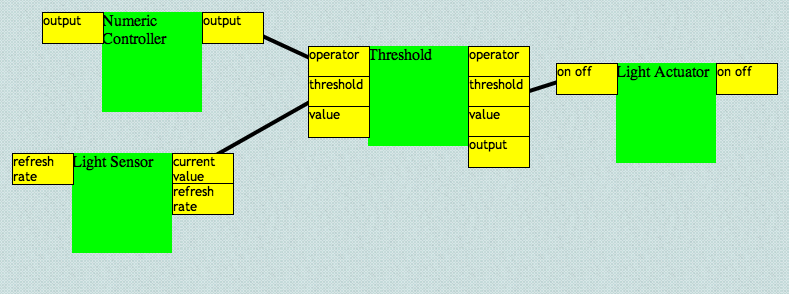
\includegraphics[width=\linewidth]{figures/fbp-application}
\label{fig:fbp-application}
\end{figure}

M2M applications are by definition distributed where the application
requirements involve a network of nodes collaborating for some common 
goals. M2M applications are typically defined by its flow of information
between components, as opposed to more traditional applications that focus more
on local information processing.

Flow Base Programming is best suited for describing M2M applications as it
allows the developers for the applications to focus more on the
abstraction meaning of the components instead letting the unimportant details
such as the hardware to stick right in the face. The result application will
contain all necessary information for the framework to construct low-level
details to implement the flow.

Applications are designed and constructed on FBP canvas by dragging a set of
abstract components from the library as illustrated in Figure~\ref{fig:fbp-application} 
Each component is
illustrated by a green block, each block has a set of properties, each with
different access modes, such as readonly, writeonly, readwrite. Properties on
the left of the greenblocks are properties that could be written, and
properties on the right are readable. Components are connected by links, which
is drawn by linking two properties in different components.

Some components represent physical hardware such as a sensor, or an actuator
while some other components could represent virtual processes such as
mathmatical computations, comparisons, etc. However, the final physical implementations
of the components are only made during application deployment by the Master but
not during FBP construction.

Components expose their interface through properties. A link is only made with
properties with matchinkg data type. The FBP applciation in
Figure~\ref{fig:fbp-application} illustrates a simple scenario where the light actuator
will turn on the light if light level drops below some value. The Numeric
Controller component will be assigned to a user input device used by users to
set its desire light threshold, which its output is sent to Threshold
component. The light value is sensed from Light Sensor component and sent to
Threshold. If the light value sensed is below the threshold value, Threshold
will output a boolean to set the on off property of Light Actuator to turn the
device, which will be deteremined during deployment, that it is represented by
on or off.

\subsection{Sensor Profile Framework}

While FBP defines the logical view of an application, WuKong profile framework allows
tracking, identification of physical resources within the Sensor Network.
There are a range of sensors which provide similar functionality with different
level of quality, it could model the sensor capability to enable handling
heterogeneous sensors and provide a common abstraction for the logical view.

There are two main concepts in Sensor Profile Framework, WuClasses and
WuObjects. WuClasss model components by exposing a number of properties
describing, and allow access to, a specific resource represented by the class.
Drawing from the example in Figure~\ref{fig:fbp-application}, the on off property of Light
Actuator component is boolean writeonly. WuClass also implements an update()
function to describe a component's behavior. For
example, Threshold has four properties: operator, threshold, value, output. The
output value is determined from the previous 3 properties that it returns true
when the value is lower or higher than the threshold which depends on the value
of the operator, and it returns false otherwise.


WuObjects are the main unit of processing that are hosted on the nodes. Each
WuObject is an instance of WuClasses. It allows the framework to achieve
4 responsibilities:
\begin{enumerate}
\item Allow the Master to discover the current status of a node with the list
of WuClasses and WuObjects it has.
\item Create new WuObject instances on a node to start receiving data and doing
local data processing.
\item Trigger executions in WuObjects, either periodically or as a result of
changing inputs.
\item Propagate changes of properties between linked properties in different
components, which may be hosted locally or remotely.
\end{enumerate}

\subsubsection{Property Propagation}

The profile framework is in charge of communication between WuObjects as
well, which are not necessarily on the same nodes. Profile Framework monitors
the changes in properties and propagate the changes to the connected WuObjects.
For example, if a Temperature WuObject is connected to a Threshold WuObject,
the changes in Temperature current value property will trigger propagation from
the Profile Framework to propagate the new value in current value to the
Threshold WuObject connected property, and since Threshold WuObject could be on
a different node, the framework will take care of this by initiating
a wireless connection between the nodes to send the data over. Once a new value
has been set, Threshold WuObject will also trigger its update() function to
recompute its output properties which in turn would cause another chain of
propagation to the linked WuObjects.

\subsection{Compilation and Mapping}

\begin{figure}[h!]
\caption{WuKong application build flow}
\centering
    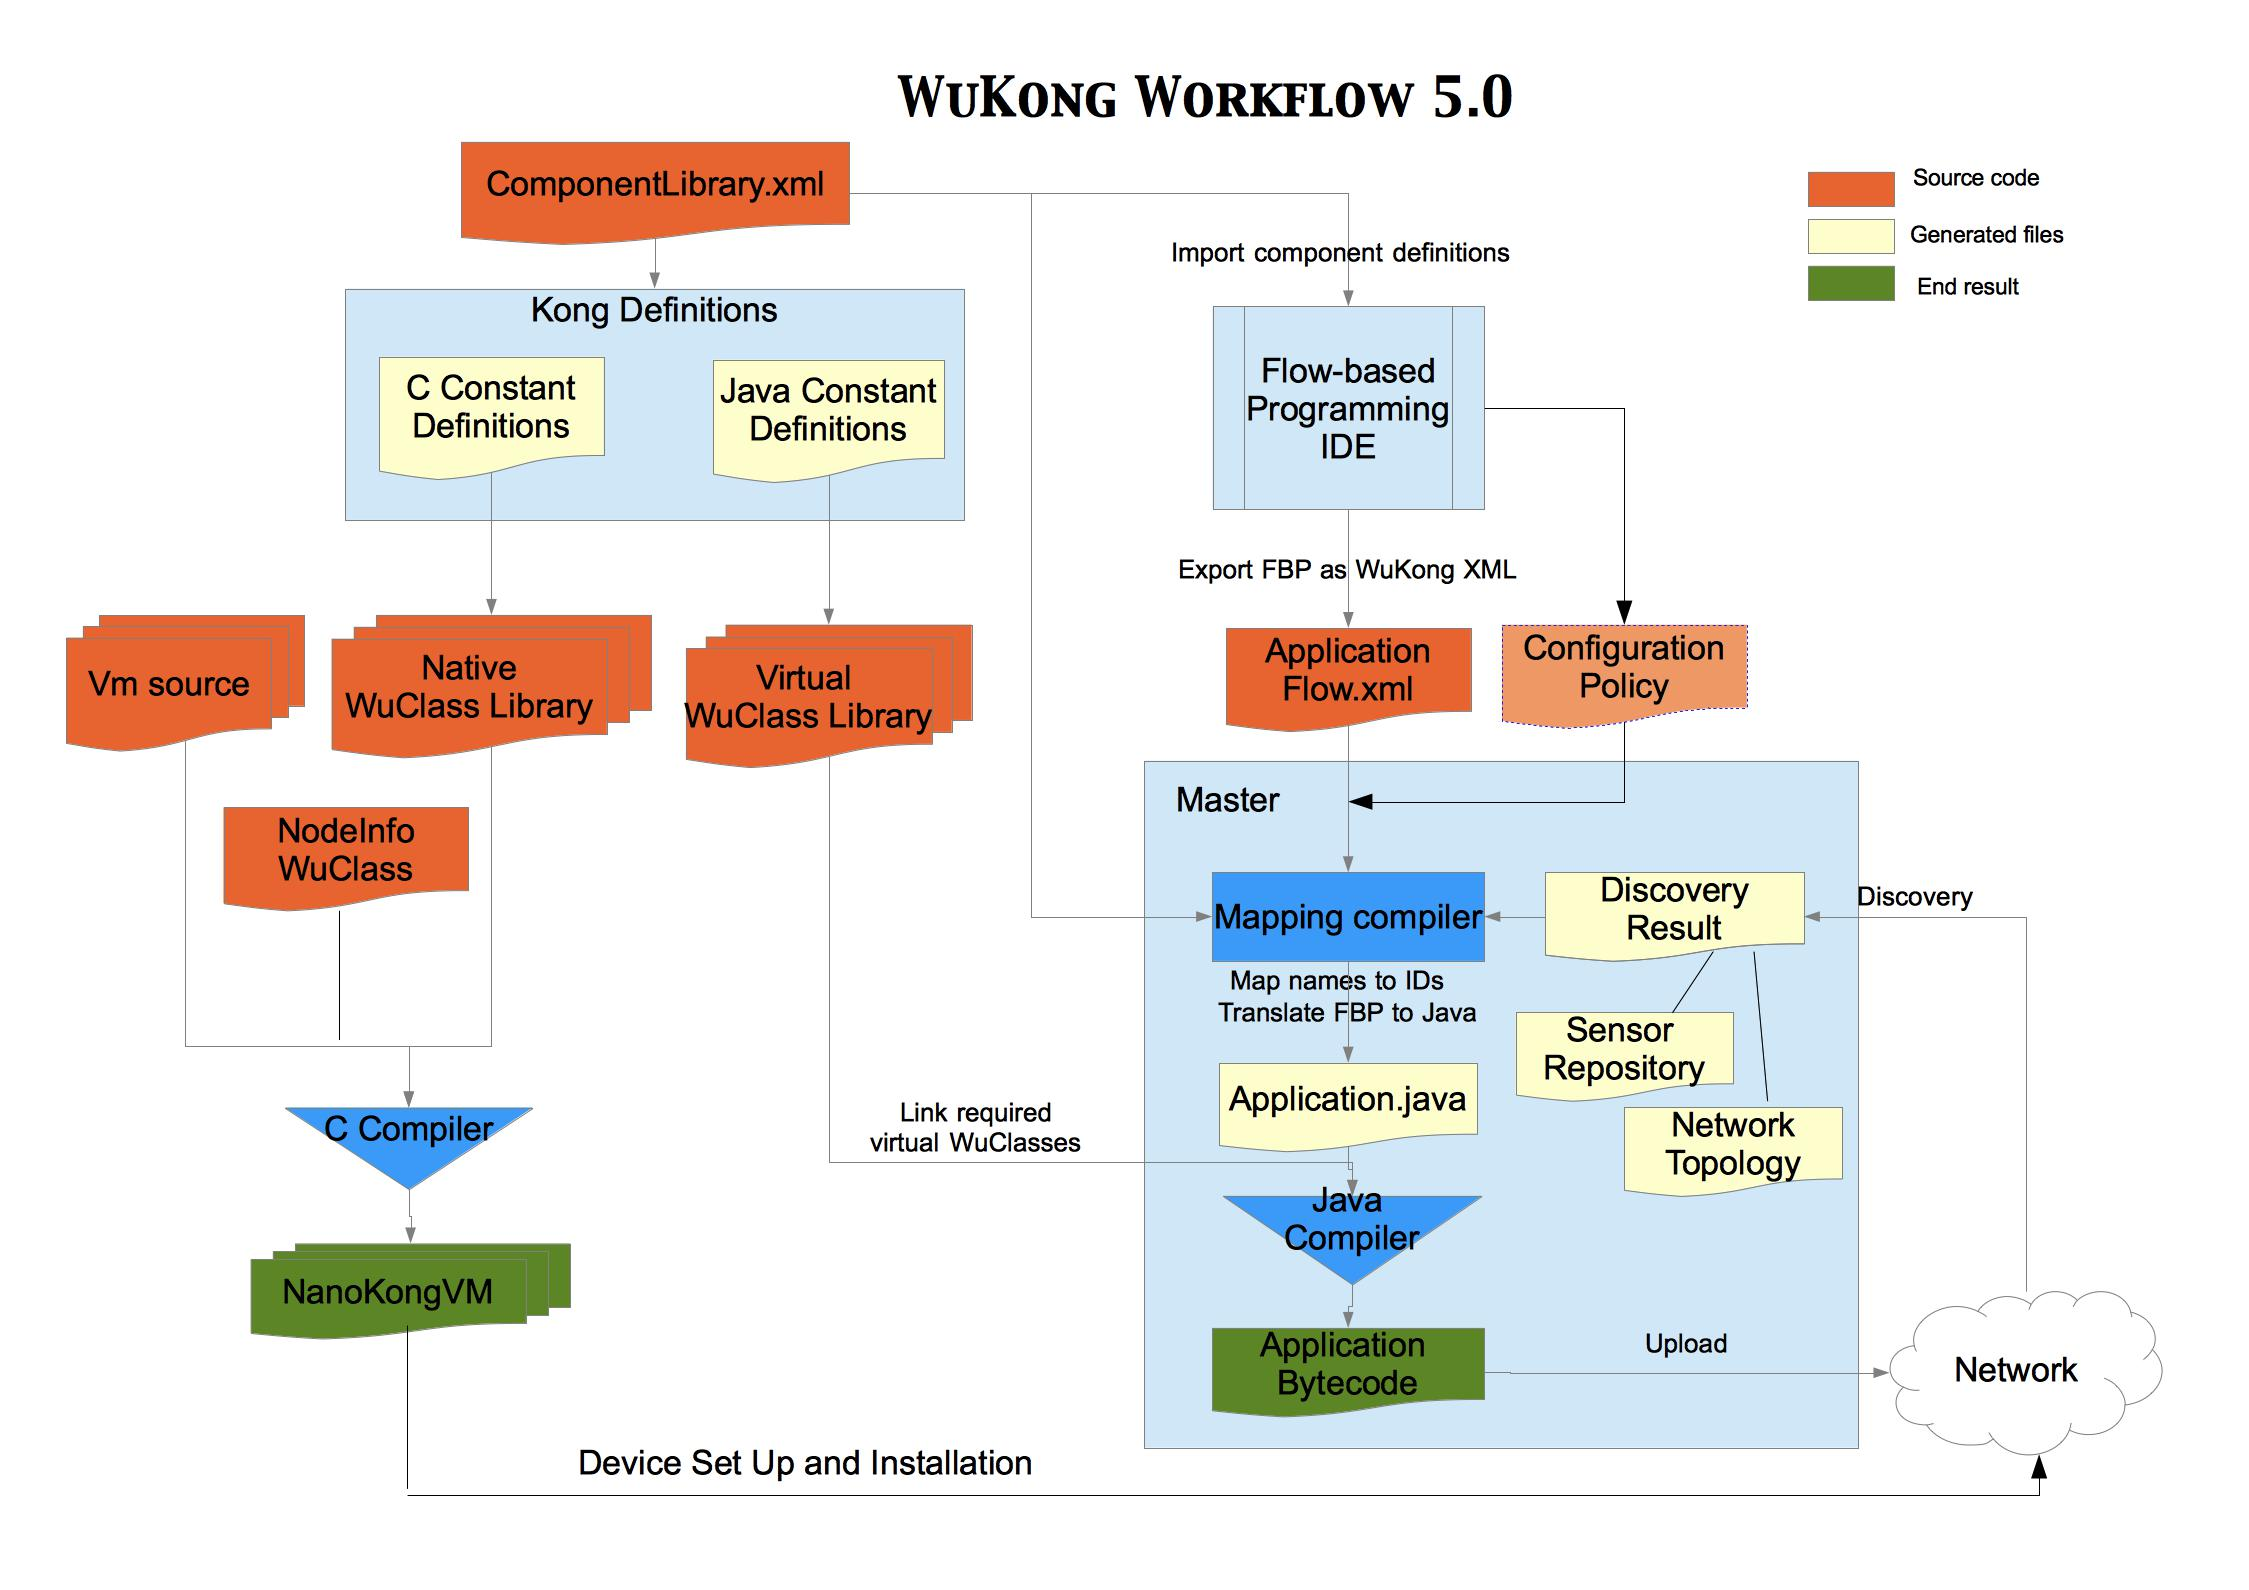
\includegraphics[width=\linewidth]{figures/wukong-flow}
\label{fig:wukong-flow}
\end{figure}

Figure~\ref{fig:wukong-flow} shows the overview of WuKong's build flow. The
left part represents the build process for NanoKong VM which will be installed
on the sensor nodes as part of the WuKong framework. The top part represents
the build process for generating component libraries and Virtual WuClass
library which will be used in other parts of the process. The right part
illustrates the build process for FBP applications from being drawn in the IDE
to Java bytecode that will be transmitted to the nodes.

The FBP program from the IDE will be exported as XML to the Master, the Master
will then take this XML and passed to Mapper to generate a Java program that
will be executed on the nodes. Finally, the compiled code is then wirelessly
uploaded to the nodes in the network.

The Java code consists of many parts from different phases of the mapping process.
First, the Java code contains information about links between components that
were taken from the FBP XML passed in earlier from the IDE. A link contains the
source component id, destination component id. The library code for components
corresponding to the component ids are stored in the node if it is written in
native language, or uploaded as part of the Java bytecode if it is written in
Java language. Second, it contains information about the mapping from
application component ids to actual node identifications and positions. The
purpose of a mapping which separates from the actual link makes it easier to
substitude the actual host of the WuObject later during
reconfiguration from the Master. This mapping is created by the Master during
discovery phase that probe the network for node's capabilities in terms of
available WuClasses, then mapper will decide the final candidates that will be
hosting for a component. If no native version of a component is found on the
nodes, mapper will substitute with a Java version of it.

\subsection{System Progression Framework}

There are a few popular wireless communication protocols in M2M applications:
ZigBee, ZWave. It is expected that in the future more diverse
wireless nodes equipped with radios that support protocols such as low-power
bluebooth and WiFi that all have one or more powerful gateway to connect to the
outside world. In WuKong system, one of the gateways will take on the role of
higher management decision maker called \emph{Master} to making the decisions for
deployment and producing the configuration of wireless sensor networks.

% TODO:probably need more here

\subsection{User Policy Framework}

\begin{figure}[h!]
\caption{A user component policy dialog}
\centering
    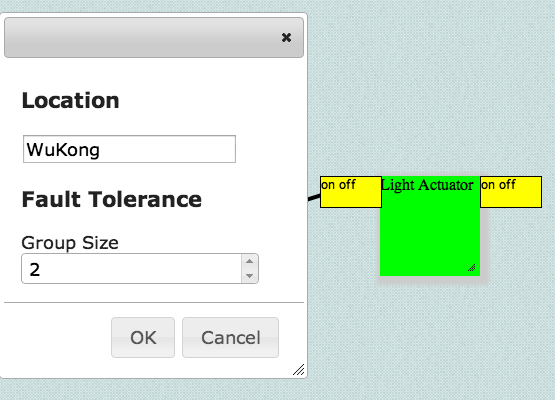
\includegraphics[width=\linewidth]{figures/fbp-policy}
\label{fig:fbp-policy}
\end{figure}

Many M2M applications are heavily influenced by user preferences and current
environmental context, as users and objects are mobile and application
requirements and policy could change in time. Users are able to specify
user policy for every component in the FBP and the application as a whole as
illustrated in Figure~\ref{fig:fbp-policy}

\subsubsection{Fault Tolerance policy}

M2M applications are inherently distributed, and hence it is inherently prone
to failures since all nodes are running autonomously unattended for a long
period of time where the external enviornmental influences could break and shut
down the devices easily. Fault Tolerance policy enables users to specify
relevent policy for tolerating failures in the granular level. This thesis will
discuss more on fault tolerance policy in the following chapter.

\cleardoublepage
\singlespacing
\chapter{Reconfigurable Atomic Service for Component Objects}
\label{c:rasco}
\doublespacing\nointerlineskip

This chapter presents the Reconfigurable Atomic Service for Component Objects,
RASCO in short. First, the profile framework is described in section~\ref{s:pf}.
Section~\ref{s:ss} describes a new replicas configuration models called strips
to track and handle replicas dynamically. After that section~\ref{s:dfd},
~\ref{s:fr} and ~\ref{s:reconfig} presents the distributed algorithm used to
solve the problem. The models and algorithms are tested extensively on various
benchmarks, described in section~\ref{s:benchmarks}, and the results are
discussed and compared with existing fault tolerant system models in
section~\ref{s:results}

\section{Profile Framework}
\label{s:pf}

In this work, we build upon WuKong, a loosely-coupled component based
architecture for M2M systems. WuKong uses profile
framework to enable the handling of physical resources on heterogeneous sensor
nodes, and for higher abstractions of software component capabilities. As
future M2M systems could consist of many heterogeneous sensor nodes and
actuator nodes, two main concepts in profile framework, namely WuClass and
WuObject, was introduced to allow WuKong to track, and manage physical
resources in the network.~\cite{Reijers} However WuKong has no support for
fault tolerance. We proposed a solution to track, manage and maintain
consistency among replicas based on concepts of WuClasses and WuObjects from
profile framework. Replicas replicate WuObjects, such as WuClass ids but not
their respective ports on their respective hosts, and link information. Among
the hosts that have the same WuObjects, only one is active and is the primary
service provider in the eyes of other services and clients.

\section{Strips} % good name?
\label{s:ss}

\begin{figure}[h!]
\caption{An example network with several strips}
\label{fig:strips-network}
\centering
    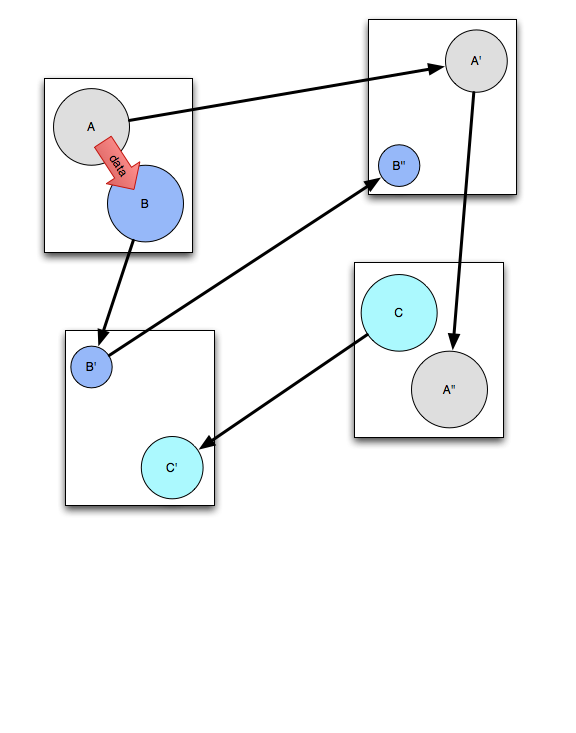
\includegraphics[width=\linewidth]{figures/strips-network}
\end{figure}

This work proposed an algorithm that uses strips. Strips are a sequence of
WuObjects on different nodes where the node holding the first WuObject is
active in the system while the rest are backups. The order of a strip is
typically determined by the system that deploys the application. Strips
consists of members which are chained together in series to the next that when
one member failed, the next one will take over, except the last one. For
example, for a strip constructed like this $\rightarrow 1-2-3-4-5$, when
3 failed 4 will take over the place of 3 and shift all the objects after it
forward, and the new chain will look like this: $\rightarrow 1-2-4-5$. Now if
1 failed, 2 will take over and members after 2 (including 2) will shift one
position forward that would result in $\rightarrow 2-4-5$. When a backup
becomes the head of the strip, it will become active in the system.

In a heterogeneous network, each host could carry more than one WuObjects.
Since each strip represents a specific component in the application, there will
typically be many of these strips present in the network where each of them
could crisscross with one and others. So it is typical that a node could be
carrying inactive WuObjects and active WuObjects at the same time.

A node stores membership information of the strips where it is a member of. As
later sections will also introduce to the heartbeat protocols that each node will
be monitoring some other nodes, each node will also store the membership
information of the strips of the nodes it is monitoring. Each stripe is stored
as a list with membership address information in the same order as the order of the
strips so for example, the current head of the strip is the first element of
the list. Nodes use the information stored to track and notify the nodes for
any changes in the strips.

Figure~\ref{fig:strips-network} illustrates a network with many strips as
strips crisscross and layout in the network. Each block represents a host, and
each circle is a WuObject. Notice that only the head (one with no arrows
pointing at) of the strip is active. The name of the component represents the
type of the component, and replicas have the same name as the component but
with an apostrophe next to it. As shown in the figure, each strip could
crisscoss and could have replicas residing with another component within the
same host.

\section{Decentralized Failure Detection}
\label{s:dfd}

The system assumes a fully connected heterogeneous network with sensors and
actuators where each node in the network could host multiple components. This
work uses heartbeat technique, a popular technique widely used to detect
failures in high-availability distributed systems. Each node would send
a heartbeat message to its detector periodically in a fixed interval
until it's unable to send messages anymore. Each node is therefore suspected
dead when it stops sending messages after a period of time.

There are many related work on heartbeat protocols to ensure high-availability
whether it uses star topology, or a ring topology; the main purpose for
a heartbeat protocol is to detect failure within a network as fast as possible.
Our work assumed a ring topology heartbeat protocol such that a node A would
send heartbeat to node B and so on, but the last node would send heartbeat back
to node A.

However, the heartbeat protocol used in the network is not directly related to
the ordering of the strips. The heartbeat protocol is a layer below the strips
as a support for network fault detection, the algorithm above will take
advantage of the given information from the layer below to recover the system.

\section{Failure Recovery}
\label{s:fr}

When a failure is detected, there are two tasks that the system will have to do
to recover from failures. First it has to maintain membership consistency among
affected strip members. Second, it would need to propagate the changes to
reconfigure other parts of the system that depend on the locations of the heads
of the affected strips in order to function. The work built on a stateless
system as defined by WuKong middleware with FBP applications where none of the
services need to store any states or to remember any history. For example,
WuKong applications don't have services that require to store past values of
some variables. Therefore strips members (except the head) with inactive
WuObjects are not the same replication as defined in other related work, but
simply as backups that will take over when the active WuObject failed.


% should state stateless distributed system to enable no replication in the
% sense of other related work

% should also state how it is stateless, and how it is different from other
% distributed systems

\subsection{Consistency within strip members}

Typically several strips would be cut off in the event of failure, and if the
failed node carries some active WuObjects from some strips, the system would
not able to continue to function. RASCO will attempt to recover by letting the
detector of the failure to initiate the recovery algorithms.
Since the detector will be responsible for recoverying for the failed node,
every node needs to have membership knowledge of the strips from the nodes it
is monitoring. For example, if node A is monitoring node B, A would know the
members of all strips in node B in addition to its local strips. Strips only
specifies the order of recovery, it is not correlated with the network
structure for the fault detection, in other words, a strip with A and B doesn't
mean B is monitoring A, as B could be monitored by C which depends on the
structure of heartbeat protocol layer.
In the initial algorithm, the detector node will prepare a update message to
inform all members of the strips with which the failed node is associated with.
Assuming that every node that monitors other node will have knowledge of the
strips that it contains and the members that the strips pertain. The node would
send out a marker multicast first to confirm the nodes which are still
functioning, and once all acknowledges have been received, it will proceed to
send the update message to update their local knowledge of the strips to reach
a consensus. The ordering of the messages wouldn't matter since the end state
of any failure sequence for any strip would be the same. For example, given
a strip of three members $\rightarrow 1-2-3$, if the updated failure sequence
is given in any permutation by $[1, 2]$ or $[2, 1]$, the end results would be
the same $\rightarrow 3$ since the remaining members from those two failure
sequence is the same and the relative order of the members would stay the same.
\begin{comment}
Let's assume there is a pair of failure patterns with the same members but
different orders that would do update operations on the same strip but would
leave the strip in different results. If that's true, then by building back the
strips from the result in the order of update operations would result in
a different starting state, that implies the strips have different members or
member orders to start with, a contradiction.
\end{comment}
Therefore there is no need for extra communication overhead to maintain
ordering to gaurantee level of consistency between members since they will all
come to the same conclusion given each receiver receive the same messages.

% performance? complexity analysis?

\subsection{Reconfiguration}
\label{s:reconfig}

Even though consensus of the new configuration for each affected strip has been
reached, some nodes with component that acts as a client to another component
for data or the reverse would also have to have consensus on the updated
primary holder of each affected component. And the node that is monitoring the
node monitored by the dead node would also need to update on its knowledge of
its monitored node in order to recover the next possible failure.

RASCO will initiate a reconfiguration service to reconfigure the network to adapt
to the new strip configurations. Reconfiguration service is implemented by
a distributed algorithm which is inititated by the detected nodes. First the
initiator node would have to identify the components that are reading/writing
data with the components carried by the dead host. This would be done by
requesting the link information between components at the higher level provided
by the application. Then each member of the strips of the connected components
would be updated with the information about the change in the host of the
failed components with a \emph{reconfig} message containing the change in the
location of the specific WuObjects. Right after receiving the \emph{reconfig}
message, if the connected nodes whose WuObjects are pushing data to the
WuObjects on the failed nodes, they will force to initiate a data push to
update and bring the recovered nodes up to date, and vice versa, so the nodes
whose WuObjects are receiving data from the failed nodes will initiate a data
pull after receiving the \emph{reconfig} message.

% remember also to state the important of reacting the other hosts with
% connected WuObjects to push or pull to get the new head to get to the last
% valid state

% state clearly what happened, for each case, push or pull


Reconfiguration service has message complexity of $O(m)$ where m is the
number of strips where its components are linked to the failed components.

\begin{comment} % temporarily
\section{Benchmarks}
\label{s:benchmarks}

% here states that we deployed on wireless sensor platform for proving that it
% works for the most resource limited distributed platform

\subsection{Implementation}

\subsubsection{Setup}

\subsubsection{Hardware Platform}

All boards are equipped with an Atmel ATmega1280-16AU 8-bit microcontroller with 4K of EEPROM and 64k of flash. The boards hardware design is based upon Arduino hardware referenced design, in addition, every board has wires for mounting multiple wireless protocol adapters such as ZWave, ZigBee. In the following experiments, every board is only equipped with a ZWave adapter, and only communicating through ZWave. 

Every board is also pre-installed with a modified version of NanoVM (ref here) called “NanoKong” that supports all the basic WuKong framework protocols including the new additions from the work in the previous chapter.

A PC with wireless access is dedicated for hosting the WuKong Master software which is responsible for managing WuKong applications for the whole system and serves as a mean to present an interface to the users.

Three boards will be used in the experiments below. One of them is equipped with a light sensor that returns a byte indicating the light level around the sensor. The rest are equipped with a relay which each controls the power supply of a lamp.

An additional board with the same hardware specification is used as a gateway between the Master and the sensor network.

\subsubsection{Heartbeat Daisy Chains}

\subsubsection{Strips}

\section{Experimental Results}
\label{s:results}


%Describe limits: 
%1. Fully connected network

\section{Experiment - Application Deployment}

To evaluate the performance of the result of the new mapping algorithm and the overall fault tolerant framework, an application shown in Figure 1 will be deployed.

\subsection{Experiment Design}

In this experiment, an application shown in figure 1 above will be deployed with a fault tolerance user policy shown in the figure 2 upon the hardware setup described in the previous section three times to evaluate its performance.

The application requires a light sensor and a light actuator. The light actuator will turn on the light if the sensed light value is below a threshold specified from the numeric controller. Numeric controller is fixed on a value of 200. The light value takes a byte ranging from 0 to 255. The comparison is done with a virtual component Threshold in native implementation.

We will simulate a node failure by unplugging the power supply of the active light sensor node on all tries.

\subsection{Experimental Result}

The performance of the fault tolerance system is evaluated with the metrics listed below:
\begin{enumerate}
\item Correctness, whether the system is configured to do what the mapping result specifies, including the heartbeats, heartbeat periods, recovery chains, application links.
\item Communication overhead used for heartbeats
\item Communication overhead for failure recovery
\item Failure detection success rate
\item Fault recovery success rate
\item The average time to recover from the time of failure
\item The average number of messages used to recover the system
\end{enumerate}
\end{comment} % temporarily

\cleardoublepage
\singlespacing
\chapter{Deployment of Reconfigurable Atomic Service for Component Objects}
\label{c:deploy}
\doublespacing\nointerlineskip

\begin{comment}
Niels:about the tradeoffs in determining the deployment from your fault
tolerance perspective
\end{comment}

\section{Reconfigurable Atomic Service for Component Object}

\begin{comment}
Niels suggested that I show that I am aware of such issue with determining
optimality for deployment which is not clear for WuKong yet, there are many
ways or metrics to optimize for, all I can do in this work is to identify some
tradeoffs certain deployment for fault tolerance could influence the system
with certain metrics.

Limits will be hard to define here
\end{comment}

\section{Policy Framework}

\subsection{Fault Tolerance Policy}

\section{Set Covering Problem}

% http://www.cs.dartmouth.edu/~ac/Teach/CS105-Winter05/Notes/wan-ba-notes.pdf

\section{Greedy Approximation Method}

\section{Hybrid Method}

\section{Discussion}

\cleardoublepage
\singlespacing
\chapter{CONCLUSION}
\label{c:conclusion}
\doublespacing\nointerlineskip

%Previous chapters have described the work that has been done on WuKong platform.
%It is useful to reflect on what has been accomplished and place them in the
%broader context of the more general fault tolerance problem as well as the
%specific contributions of this work.

\section{Discussion}

This thesis proposed a novel algorithm to achieve
recovery from failures by combining heartbeat protocol, for failure detection,
with Strips, which are used to maintain and track service redundancy.

We have presented a fault tolerance system able to provide failover for failed
services in service-oriented WSNs that comply with user policy requirements. We
have also described strip, a redundancy abstraction for service peers along with
distributed algorithms to synchronize strip views among members and
reconfigurate the network for the new structure to recover from node failure.
The system allows user intervention through means of user policy, which could
directly influence underlying system configurations and structure.

The developed methods add new and useful solutions to build a fault tolerant
system that could be reasoned easily and with a performance as expected on
average. This method makes an extension to other methods in terms of
completeness and complexity. It serves as a quick and easy solution
to provide practical fault tolerance for WuKong applications.

% TODO: summarize the results of the experiments here, etc
% e.g. The solutions developed for WuKong system performs very consistently, as
% the recovery time is always under two secs on average with a handful of
% sensors. However, occationally heartbeats could report erroneous failures and
% result in a quick false recovery, and left the partitioned nodes behind, but
% the system as a whole still function properly.

The experimental results have shown to be consistent and stable among first
failures in different rank of members in strip around 2.5 secs. The failover
have been successful in all deployments. It is also shown that the performance
degraded quickly when the hardware or the wireless communication quality
degraded. Therefore it is important that the network setup is as optimized as
possible. 

\section{Future Work}

% Probably move it to future work? Probably don't do it.
%Of course there are a lot of room for improvements. For example, if we want to
%go beyond this limitation of 232 nodes by Zwave, one of the ways we could do is
%to build another zwave network and have a routing agent to route messages
%between networks. And we would also want to handle network partitions. One of
%the possible research directions is to merge the partitions back to one if they
%come back together, or by using some arbitrary flags to indicate primary
%components in the network to eliminate redundant commanding network components.
%Nonetheless, it is also an opportunity to look into multi-hop networks since
%heartbeats protocols are designed with single-hop network in mind, whether we
%could change the protocol to handle multi-hop is also a big challenge a future
%research could take on.


We have shown a design for a reconfigurable fault tolerant system for WuKong.
Strips makes it really easy to describe a component system with redundancy for
heterogeneous services and devices. Nevertheless, there is still room for
improvements. This section will address some directions future research can take.

WuKong Fault Tolerance System did not consider for network partition. Network
partition occurs when a network of nodes got partitioned into two subnetworks where
none can detect each other for a period of time. One of the possible direction
is to create a more sophisticated failure model that could handle network partition.
In this thesis we assume failstop model where nodes, once dead, will not come
back. Therefore when network partition occurs, each part of the network would
not be able to recognize each other and would cause conflicts and confusions.

Our current heartbeat protocol is distributed and easy to construct, but it is
not shown to work under networks where messages are sent in multiple hops, since
the algorithm used to produce where each node should be sending heartbeat
messages does not consider the topology of the network. Heartbeat is sensitive
on latency, so if a heartbeat message was not received within tolerance period,
a failure event could occur and the node is suspected of failure and will
never come back. If the node is still alive, it would be treated as if it is
dead. And that will creates an artificial network isolation where a few nodes
are excluded from the network before of latency.

Current system can only allow the detector to handle one failure at a time. It
would be a desirable future research direction to investigate handling
consecutive node failures. One possible way is by storing ahead multiple nodes'
strips and heartbeat protocol data, such that when consecutive nodes failure
occurred the detector would be able to recover those services it backed up.
However there is a tradeoff on the memory a node could store and the number of
consecutive node failures a network could handle.

\begin{comment}
Niels suggested that I show that I am aware of such issue with determining
optimality for deployment which is not clear for WuKong yet, there are many
ways or metrics to optimize for, all I can do in this work is to identify some
tradeoffs certain deployment for fault tolerance could influence the system
with certain metrics.

Limits will be hard to define here
Niels:about the tradeoffs in determining the deployment from your fault
tolerance perspective
Penn:Remember what the prof told me, about policy, first fit, last fit, etc
\end{comment}

The optimization problem for application deployment is also an important element
in this system. This thesis didn't consider finding a optimal deployment for the
level of redundancy specified in the user policy. The problem of deploying
a specific distributed system onto a network structure typically consists of
mapping the components of the system onto the hosts of the network. The mapping
is subject to constraints. The constraints could be whether a node supports
certain service to host certain components, and how much communication overhead
would induce from the assignment to maintain consistency for the strips, and
from the perspective of WuKong, some components need to seaparate from other
components to achieve fault tolerance, and some needs to place together to
function properly.  Determining such an optimal deployment is a combinatorial
optimization problem, and combinatorial optimization problems generally
extremely challenging computationally. It is difficult to predict what will and
what will not work.  It is unlikely that a single approach will be effective on
all problems or instances of the same problems. As we also want the system to
come up with a solution within a time limit. So finding a good balance between
the quality of a solution of the time it takes to come up with a good enough
solution is critical.


\backmatter

\addcontentsline{toc}{chapter}{\bibname}
\bibliographystyle{abbrv}

% input your reference here
%\bibliography{thesis}
\bibliography{/Users/penn/Documents/Bibtex/Thesis.bib}

\appendix

\end{document}
